% Options for packages loaded elsewhere
\PassOptionsToPackage{unicode}{hyperref}
\PassOptionsToPackage{hyphens}{url}
\PassOptionsToPackage{dvipsnames,svgnames,x11names}{xcolor}
%
\documentclass[
]{article}
\usepackage{amsmath,amssymb}
\usepackage{iftex}
\ifPDFTeX
  \usepackage[T1]{fontenc}
  \usepackage[utf8]{inputenc}
  \usepackage{textcomp} % provide euro and other symbols
\else % if luatex or xetex
  \usepackage{unicode-math} % this also loads fontspec
  \defaultfontfeatures{Scale=MatchLowercase}
  \defaultfontfeatures[\rmfamily]{Ligatures=TeX,Scale=1}
\fi
\usepackage{lmodern}
\ifPDFTeX\else
  % xetex/luatex font selection
\fi
% Use upquote if available, for straight quotes in verbatim environments
\IfFileExists{upquote.sty}{\usepackage{upquote}}{}
\IfFileExists{microtype.sty}{% use microtype if available
  \usepackage[]{microtype}
  \UseMicrotypeSet[protrusion]{basicmath} % disable protrusion for tt fonts
}{}
\makeatletter
\@ifundefined{KOMAClassName}{% if non-KOMA class
  \IfFileExists{parskip.sty}{%
    \usepackage{parskip}
  }{% else
    \setlength{\parindent}{0pt}
    \setlength{\parskip}{6pt plus 2pt minus 1pt}}
}{% if KOMA class
  \KOMAoptions{parskip=half}}
\makeatother
\usepackage{xcolor}
\usepackage{color}
\usepackage{fancyvrb}
\newcommand{\VerbBar}{|}
\newcommand{\VERB}{\Verb[commandchars=\\\{\}]}
\DefineVerbatimEnvironment{Highlighting}{Verbatim}{commandchars=\\\{\}}
% Add ',fontsize=\small' for more characters per line
\newenvironment{Shaded}{}{}
\newcommand{\AlertTok}[1]{\textcolor[rgb]{1.00,0.00,0.00}{\textbf{#1}}}
\newcommand{\AnnotationTok}[1]{\textcolor[rgb]{0.38,0.63,0.69}{\textbf{\textit{#1}}}}
\newcommand{\AttributeTok}[1]{\textcolor[rgb]{0.49,0.56,0.16}{#1}}
\newcommand{\BaseNTok}[1]{\textcolor[rgb]{0.25,0.63,0.44}{#1}}
\newcommand{\BuiltInTok}[1]{\textcolor[rgb]{0.00,0.50,0.00}{#1}}
\newcommand{\CharTok}[1]{\textcolor[rgb]{0.25,0.44,0.63}{#1}}
\newcommand{\CommentTok}[1]{\textcolor[rgb]{0.38,0.63,0.69}{\textit{#1}}}
\newcommand{\CommentVarTok}[1]{\textcolor[rgb]{0.38,0.63,0.69}{\textbf{\textit{#1}}}}
\newcommand{\ConstantTok}[1]{\textcolor[rgb]{0.53,0.00,0.00}{#1}}
\newcommand{\ControlFlowTok}[1]{\textcolor[rgb]{0.00,0.44,0.13}{\textbf{#1}}}
\newcommand{\DataTypeTok}[1]{\textcolor[rgb]{0.56,0.13,0.00}{#1}}
\newcommand{\DecValTok}[1]{\textcolor[rgb]{0.25,0.63,0.44}{#1}}
\newcommand{\DocumentationTok}[1]{\textcolor[rgb]{0.73,0.13,0.13}{\textit{#1}}}
\newcommand{\ErrorTok}[1]{\textcolor[rgb]{1.00,0.00,0.00}{\textbf{#1}}}
\newcommand{\ExtensionTok}[1]{#1}
\newcommand{\FloatTok}[1]{\textcolor[rgb]{0.25,0.63,0.44}{#1}}
\newcommand{\FunctionTok}[1]{\textcolor[rgb]{0.02,0.16,0.49}{#1}}
\newcommand{\ImportTok}[1]{\textcolor[rgb]{0.00,0.50,0.00}{\textbf{#1}}}
\newcommand{\InformationTok}[1]{\textcolor[rgb]{0.38,0.63,0.69}{\textbf{\textit{#1}}}}
\newcommand{\KeywordTok}[1]{\textcolor[rgb]{0.00,0.44,0.13}{\textbf{#1}}}
\newcommand{\NormalTok}[1]{#1}
\newcommand{\OperatorTok}[1]{\textcolor[rgb]{0.40,0.40,0.40}{#1}}
\newcommand{\OtherTok}[1]{\textcolor[rgb]{0.00,0.44,0.13}{#1}}
\newcommand{\PreprocessorTok}[1]{\textcolor[rgb]{0.74,0.48,0.00}{#1}}
\newcommand{\RegionMarkerTok}[1]{#1}
\newcommand{\SpecialCharTok}[1]{\textcolor[rgb]{0.25,0.44,0.63}{#1}}
\newcommand{\SpecialStringTok}[1]{\textcolor[rgb]{0.73,0.40,0.53}{#1}}
\newcommand{\StringTok}[1]{\textcolor[rgb]{0.25,0.44,0.63}{#1}}
\newcommand{\VariableTok}[1]{\textcolor[rgb]{0.10,0.09,0.49}{#1}}
\newcommand{\VerbatimStringTok}[1]{\textcolor[rgb]{0.25,0.44,0.63}{#1}}
\newcommand{\WarningTok}[1]{\textcolor[rgb]{0.38,0.63,0.69}{\textbf{\textit{#1}}}}
\usepackage{graphicx}
\makeatletter
\def\maxwidth{\ifdim\Gin@nat@width>\linewidth\linewidth\else\Gin@nat@width\fi}
\def\maxheight{\ifdim\Gin@nat@height>\textheight\textheight\else\Gin@nat@height\fi}
\makeatother
% Scale images if necessary, so that they will not overflow the page
% margins by default, and it is still possible to overwrite the defaults
% using explicit options in \includegraphics[width, height, ...]{}
\setkeys{Gin}{width=\maxwidth,height=\maxheight,keepaspectratio}
% Set default figure placement to htbp
\makeatletter
\def\fps@figure{htbp}
\makeatother
\setlength{\emergencystretch}{3em} % prevent overfull lines
\providecommand{\tightlist}{%
  \setlength{\itemsep}{0pt}\setlength{\parskip}{0pt}}
\setcounter{secnumdepth}{-\maxdimen} % remove section numbering
\ifLuaTeX
  \usepackage{selnolig}  % disable illegal ligatures
\fi
\usepackage[]{biblatex}
\IfFileExists{bookmark.sty}{\usepackage{bookmark}}{\usepackage{hyperref}}
\IfFileExists{xurl.sty}{\usepackage{xurl}}{} % add URL line breaks if available
\urlstyle{same}
\hypersetup{
  pdftitle={Git and Unix Bootcamp},
  pdfauthor={Michael Ivanitskiy (mivanits@mines.edu)},
  colorlinks=true,
  linkcolor={blue},
  filecolor={Maroon},
  citecolor={Blue},
  urlcolor={Blue},
  pdfcreator={LaTeX via pandoc}}

\title{Git and Unix Bootcamp}
\author{Michael Ivanitskiy (mivanits@mines.edu)}
\date{}

\begin{document}
\maketitle

\hypertarget{syllabus}{%
\section{``Syllabus''}\label{syllabus}}

\begin{itemize}
\tightlist
\item
  polls
\item
  introduction
\item
  installing git and bash
\item
  navigation in bash
\item
  common bash utilities
\item
  pipes, redirects
\item
  absolute basics of vim
\item
  basic introduction to git: cloning, staging, commiting, pushing,
  pulling
\item
  working with multiple people in the same git repository
\item
  GitHub-specific tools: pull requests, CI/CD
\end{itemize}

\hypertarget{quick-poll}{%
\section{Quick Poll:}\label{quick-poll}}

\begin{itemize}
\tightlist
\item
  which operating system are you currently using? (Mac, Windows, Linux)
\item
  have you used a terminal (bash, zsh, fish, cmd, PowerShell) before?
\item
  have you used an sh-compatible terminal before?
\item
  have you used git or github before?
\end{itemize}

\hypertarget{introduction}{%
\section{Introduction}\label{introduction}}

Some definitions:

\begin{itemize}
\tightlist
\item
  an \textbf{Operating System} is software that manages software and
  other hardware for a computer, and provides common services.

  \begin{itemize}
  \tightlist
  \item
    MacOS, Windows, Android, iOS, and the various Linux distributions
    (Ubuntu, Mint, Arch, etc) are all operating systems
  \end{itemize}
\item
  a \textbf{command-line shell} is a program that interprets a language
  that allows the user to have access to operating system services

  \begin{itemize}
  \tightlist
  \item
    these services include moving files around, running or stopping
    other programs, and pretty much anything you can expect to be able
    to do with a computer
  \end{itemize}
\item
  a \textbf{version control system} is responsible for tracking and
  managing changes to source code and programs. when working on all but
  the smallest pieces of code, this becomes extremely useful. Think of
  it as google docs edit history, but for source code

  \begin{itemize}
  \tightlist
  \item
    the only version control system that you should worry about learning
    is git -- for now, all others see relatively niche application in
    industry
  \end{itemize}
\end{itemize}

Now, some history:

\begin{itemize}
\tightlist
\item
  ``Unix'' is a family of operating systems, originating from Bell Labs
  in 1969
\item
  the GNU project (a recursive acronym standing for ``GNU's not Unix!'')
  was created in 1983 with the goal of giving computer users freedom in
  their use of computing devices. it has created a wide variety of
  open-source tools, including bash (Bourne-again shell) in 1989 to
  replace the original Bourne shell for Unix
\item
  ``Linux'' is a family of open-source ``unix-like'' operating systems,
  and most ``serious'' computing is done on Linux today.
\item
  ``git'' is a version control system originally created to manage the
  development of the Linux kernel, but has been widely adopted in all
  areas of software and is the de-facto standard for version control
\end{itemize}

\begin{figure}
\centering
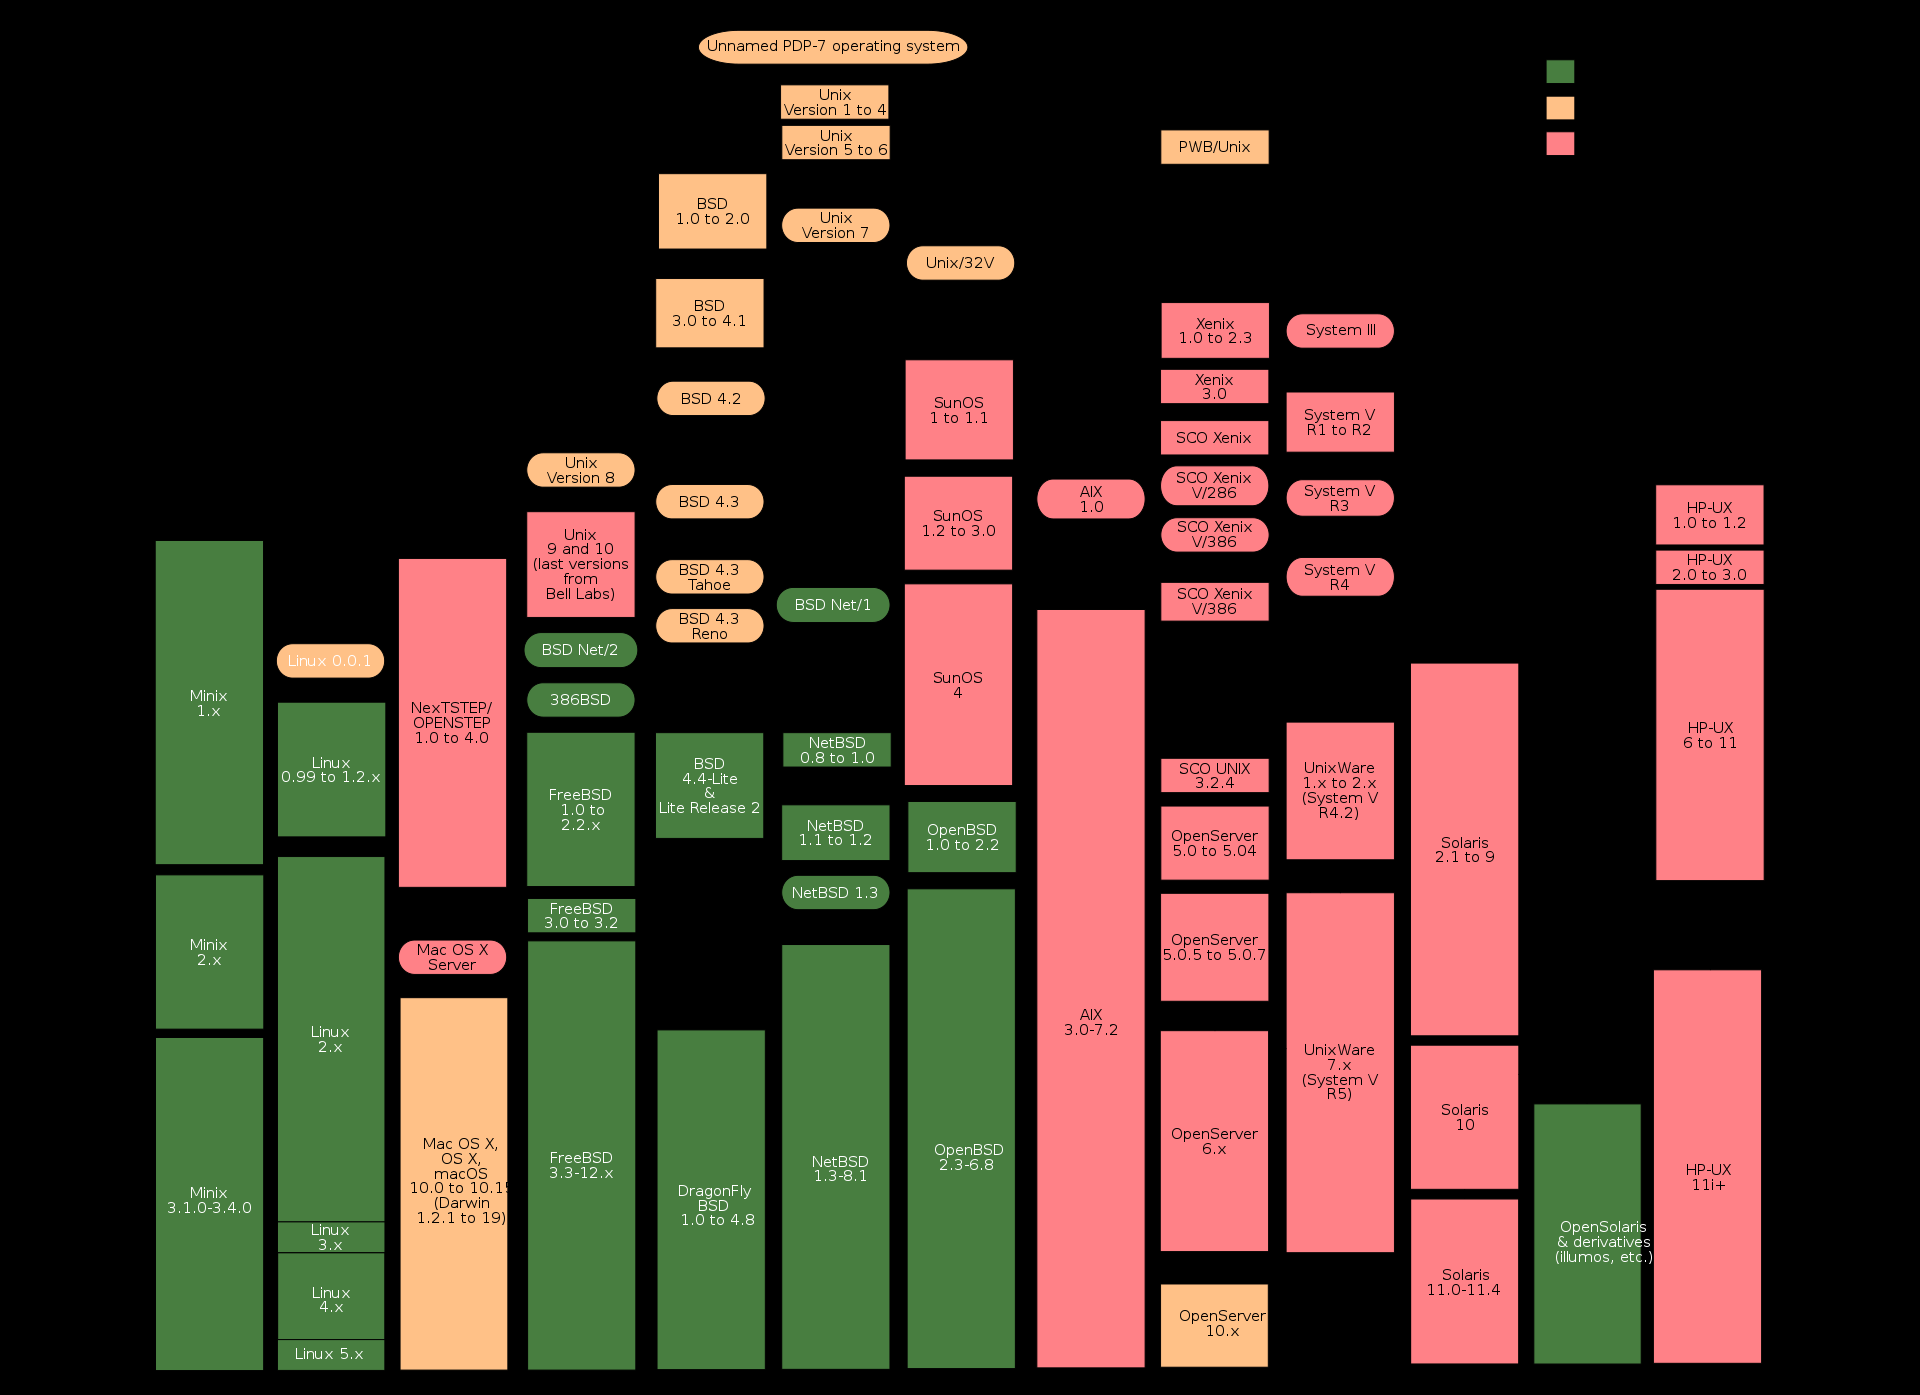
\includegraphics{images/unix-evolution.png}
\caption{Evolution of Unix and Unix like systems (credit: Wikipedia)}
\end{figure}

\hypertarget{installing-bash-and-git}{%
\section{Installing bash and git}\label{installing-bash-and-git}}

if you're prompted during installation to select a default text editor
for editing commits, I reccomend \texttt{nano}, but feel free to choose
whatever you're comfortable with

\hypertarget{macos}{%
\subsection{MacOS}\label{macos}}

\begin{itemize}
\tightlist
\item
  MacOS comes with either bash or zsh, depending on how recently you've
  updated. simply start up the ``Terminal'' program
\item
  to install git, go to \href{https://git-scm.com}{git-scm.com}
\end{itemize}

\hypertarget{windows}{%
\subsection{Windows}\label{windows}}

Windows comes with both the \texttt{cmd} shell and PowerShell, but
you'll want to install bash. Navigate to
\href{https://gitforwindows.org}{gitforwindows.org}, and download and
run the installer.

\begin{quote}
NOTE: When prompted about line endings, select ``Check out as-is, commit
LF''
\end{quote}

when the installation is complete, start up ``git bash'' from the start
menu

\hypertarget{linux}{%
\subsection{Linux}\label{linux}}

Almost all distributions of Linux come with bash or some other
sh-compatible shell, and git.

\hypertarget{testing}{%
\subsection{testing}\label{testing}}

after installing, launch your terminal, type

\begin{Shaded}
\begin{Highlighting}[]
\FunctionTok{git} \AttributeTok{{-}{-}version}
\end{Highlighting}
\end{Shaded}

and hit enter. It should print the version to the console.

now, type

\begin{Shaded}
\begin{Highlighting}[]
\BuiltInTok{help}
\end{Highlighting}
\end{Shaded}

this should:

\begin{itemize}
\tightlist
\item
  tell you what shell you're using
\item
  remind you how to use help commands
\item
  give the basic keywords of your shell language
\end{itemize}

\hypertarget{bash-basics}{%
\section{Bash Basics}\label{bash-basics}}

firstly, note that:

\begin{itemize}
\tightlist
\item
  \href{https://stackoverflow.com}{stackoverflow} is your friend!
\item
  adding \texttt{-\/-help} to almost any command will display a help
  message explaining how to use it
\item
  \texttt{*} is commonly used as a ``wildcard'' -- it will ``match'' any
  character or string of characters
\item
  text in curly braces \texttt{\{\}} will be used to mean ``replace this
  with text relevant to your usage''

  \begin{itemize}
  \tightlist
  \item
    for example, \texttt{cd\ \{path\}} changes your directory, but you
    should replace \texttt{\{path\}} with an actual path, such as
    \texttt{Downloads}
  \item
    curly braces \emph{do} have their own special meaning in bash, so be
    careful (array construction, parameter expansion, and output
    grouping. those are beyond the scope of this tutorial)
  \end{itemize}
\item
  if you get stuck in what looks like a text editor, its probably either
  \texttt{less} or \texttt{vim}. try:

  \begin{itemize}
  \tightlist
  \item
    pressing \texttt{q} (this exists \texttt{less})
  \item
    pressing \texttt{esc}, then \texttt{:}, then \texttt{q} (this exits
    vim)\footnote{\href{https://twitter.com/ctrlshifti/status/1282199281982533637}{see
      here}}
  \end{itemize}
\end{itemize}

\hypertarget{control}{%
\subsection{control}\label{control}}

\begin{itemize}
\tightlist
\item
  \texttt{ctrl+C} will close the current process
\item
  \texttt{ctrl+Z} will pause the current command, resume it in the
  background or foreground with \texttt{fg} or \texttt{bg} respectively
\item
  \texttt{TAB} will try to autocomplete a command or file
\item
  \(\uparrow\) (up arrow key) will bring up the most recent command
\item
  \texttt{ctrl+R} will search among the previous commands (this is
  \emph{very} useful)
\item
  \texttt{ctrl+A} and \texttt{ctrl+E} will bring the cursor to the start
  or end of the line, respectively
\end{itemize}

\hypertarget{navigation-file-management}{%
\subsection{navigation \& file
management}\label{navigation-file-management}}

when you run commands, it is usually important which files are around.
these commands let you move around in and modify the filesystem

\begin{itemize}
\item
  \texttt{pwd} will \textbf{p}rint the \textbf{w}orking
  \textbf{d}irectory (your current location in the filesystem)
\item
  \texttt{ls}: \textbf{l}i\textbf{s}t every file/folder in the current
  directory

  \begin{itemize}
  \tightlist
  \item
    \texttt{ls\ -al} will print it in a list format with some more data
    about the file, notable the filesize in bytes and the date on which
    it was last modified
  \item
    note that \texttt{.} means ``the current directory'' and \texttt{..}
    means ``the parent directory''
  \end{itemize}
\item
  \texttt{cd\ \{path\}} will \textbf{c}hange \textbf{d}irectory to the
  specified path
\item
  \texttt{mkdir\ \{path\}} will create a directory at the given path
\item
  \texttt{rm} will \textbf{r}e\textbf{m}ove a file (be careful!!)

  \begin{itemize}
  \tightlist
  \item
    \texttt{rm\ -rf} will remove a directory and its contents
  \end{itemize}
\item
  \texttt{cp\ \{path1\}\ \{path2\}} and
  \texttt{mv\ \{path1\}\ \{path2\}} will \textbf{c}o\textbf{p}y or
  \textbf{m}o\textbf{v}e the files specified in \texttt{\{path1\}} to
  \texttt{\{path2\}}, respectively.\\
  you can do really clever things too, like copy the contents of a
  directory:

  \begin{itemize}
  \tightlist
  \item
    \texttt{cp\ *.txt\ textfiles/} will copy all files ending in
    \texttt{.txt} into the folder \texttt{textfiles}
  \item
    \texttt{cp\ -R\ data\ moredata} will copy the contents of the folder
    \texttt{data}
  \end{itemize}
\item
  \texttt{find\ -name\ \{name\}} will find all files matching
  \texttt{\{name\}}
\end{itemize}

\hypertarget{flow-direction}{%
\subsection{flow direction}\label{flow-direction}}

in the unix philosophy, programs should input and output streams of
text.

\begin{itemize}
\tightlist
\item
  a program can read input from \texttt{stdin}, which is equivalent to
  prompting the user for some text
\item
  a program writes its output to \texttt{stdout}
\item
  a program writes any errors or warnings to \texttt{stdin}
\end{itemize}

For modern software, this isn't always the dominant paradigm, but it can
still come in handy. The following commands can be used redirecting the
outputs of a program:

\begin{itemize}
\tightlist
\item
  \texttt{\textgreater{}} redirects the \texttt{stdout} of the
  preceeding command into the file following the sign. \emph{this will
  overwrite any existing file}

  \begin{itemize}
  \tightlist
  \item
    note that anything still printed to the console is from
    \texttt{stderr}
  \end{itemize}
\item
  \texttt{2\textgreater{}} redirects \texttt{stderr} to the given file

  \begin{itemize}
  \tightlist
  \item
    can be used in combination with \texttt{\textgreater{}}:\\
    \texttt{myprogram\ \textgreater{}\ output.txt\ 2\textgreater{}\ errors.txt}
  \end{itemize}
\item
  \texttt{\textgreater{}\textgreater{}} appends the \texttt{stdout} of
  the preceeding command to the specified file, leaving the existing
  contents in place
\item
  \texttt{\textbar{}} will send \texttt{stdout} of the preceeding
  command as \texttt{stdin} to the following command
\end{itemize}

\hypertarget{utilities}{%
\subsection{utilities}\label{utilities}}

bash has many built-in programs, there are many thousands you can
install, and you can even write your own. here are a few I find myself
using regularly.

\begin{itemize}
\tightlist
\item
  \texttt{cat\ \{file\}} will print the contents of a text file to the
  console. only useful alone for short files

  \begin{itemize}
  \tightlist
  \item
    \texttt{cat\ \{file\}\ \textbar{}\ less} will open a simple viewer,
    press \texttt{q} to exit

    \begin{itemize}
    \tightlist
    \item
      (more on what \texttt{\textbar{}} does later)
    \end{itemize}
  \item
    \texttt{head\ \{file\}\ -n\ \{number\}} or
    \texttt{tail\ \{file\}\ -n\ \{number\}} will print
    \texttt{\{number\}} lines from the beggining or end of the specified
    file, respectively
  \end{itemize}
\item
  \texttt{diff\ \{file1\}\ \{file2\}} will give the difference between
  two text files
\item
  \texttt{grep\ \{text\}\ {[}filename{]}} will return lines from
  \texttt{{[}filename{]}} with \texttt{\{text\}} in them

  \begin{itemize}
  \tightlist
  \item
    this is most useful when searching for something in a file:\\
    \texttt{cat\ my\_logfile.txt\ \textbar{}\ grep\ "WARNING"}
  \end{itemize}
\item
  \texttt{tar} combines multiple files into a ``tarball'', which is a
  single file that contains multiple files within it. usage can be
  complicated

  \begin{itemize}
  \tightlist
  \item
    compressing: \texttt{tar\ -zcvf\ compressed\_files.tar.gz\ folder/}
  \item
    decompress: \texttt{tar\ -zcvf\ compressed\_files.tar.gz\ folder/}
  \end{itemize}
\item
  \texttt{gzip} compresses a single file
\item
  \texttt{nano\ \{filename\}} opens the \texttt{nano} text editor on a
  file

  \begin{itemize}
  \tightlist
  \item
    \texttt{nano} helpfully has instructions on the bottom for how to
    use it, so you're less likely to get stuck
  \item
    this is very useful for editing text files when you're connected to
    a big supercomputer without a desktop
  \end{itemize}
\end{itemize}

\hypertarget{basic-scripting}{%
\subsection{basic scripting}\label{basic-scripting}}

any command you can run in the command line, you can put in a file

\begin{itemize}
\tightlist
\item
  printing to console: use \texttt{echo\ "\{stuff\}"}
\item
  using variables: all variables in bash are strings. it's a bit weird.

  \begin{itemize}
  \tightlist
  \item
    define using \texttt{VARNAME="stuff"}
  \item
    use later by writing \texttt{\$VARNAME}
  \end{itemize}
\item
  referencing command line args: in general, \texttt{\$1} is the first
  arg, \texttt{\$2} is the second, and so on
\item
  control flow:

  \begin{itemize}
  \tightlist
  \item
    if-then blocks generally look like
    \texttt{bash\ \ \ \ \ \ \ if\ \{command\};\ then\ \ \ \ \ \ \ \ \ \ \ \{code\}\ \ \ \ \ \ \ fi}
    but the \texttt{\{command\}} can take many forms.
    \texttt{"\$VARNAME"\ ==\ "test"} will evaluate to true, but you can
    test for the existence of files and do many other things
  \item
    for loops: look them up if you must
  \end{itemize}
\end{itemize}

a simple example script:

\begin{Shaded}
\begin{Highlighting}[]
\BuiltInTok{echo} \StringTok{"you are located in:"}
\BuiltInTok{pwd}

\VariableTok{dirname}\OperatorTok{=}\VariableTok{$1}
\VariableTok{searchname}\OperatorTok{=}\VariableTok{$2}

\BuiltInTok{echo} \StringTok{"we will create and enter the directory }\VariableTok{$dirname}\StringTok{"}

\FunctionTok{mkdir} \VariableTok{$dirname} \AttributeTok{{-}p}
\BuiltInTok{cd} \VariableTok{$dirname}

\VariableTok{fname}\OperatorTok{=}\StringTok{"programs{-}}\VariableTok{$(}\FunctionTok{date}\NormalTok{ +\%s}\VariableTok{)}\StringTok{.txt"}
\FunctionTok{ps} \OperatorTok{\textgreater{}} \VariableTok{$fname}

\FunctionTok{cat} \VariableTok{$fname} \KeywordTok{|} \FunctionTok{grep} \VariableTok{$searchname}
\end{Highlighting}
\end{Shaded}

\hypertarget{system-utilities}{%
\subsection{system utilities}\label{system-utilities}}

a few commands for interacting with your operating system\\
\textgreater{} note: these work on linux/wsl, some will work on windows
with git bash, and I have no idea if they work on macOS)

\begin{itemize}
\tightlist
\item
  \texttt{ps} static process list
\item
  \texttt{kill\ \{PID\}} kill a process with the given id (use
  \texttt{ps} to get the id)
\item
  \texttt{fg} and \texttt{bg} move a process to the foreground or
  background
\item
  \texttt{top} dynamic process list, will keep updating until you do
  \texttt{ctrl+C}

  \begin{itemize}
  \tightlist
  \item
    \texttt{htop} will also display cpu utilization. useful for seeing
    if your code is actually properly parallelized, and also for looking
    kinda cool
  \end{itemize}
\item
  \texttt{sudo\ \{command\}} \textbf{DANGEROUS:} this is ``superuser''
  mode, which will let you do very dangerous things and possible brick
  your computer. use with \textbf{extreme} caution. using it on a
  cluster probably won't work and might get you in trouble
\end{itemize}

\hypertarget{using-git}{%
\section{using Git}\label{using-git}}

git is a distributed version control system. what does ``git'' stand
for? the readme of the source code states:

\begin{quote}
``git'' can mean anything, depending on your mood.

\begin{itemize}
\tightlist
\item
  Random three-letter combination that is pronounceable, and not
  actually used by any common UNIX command. The fact that it is a
  mispronunciation of ``get'' may or may not be relevant.
\item
  Stupid. Contemptible and despicable. Simple. Take your pick from the
  dictionary of slang.
\item
  ``Global information tracker'': you're in a good mood, and it actually
\item
  works for you. Angels sing, and a light suddenly fills the room.
\item
  ``Goddamn idiotic truckload of ****'': when it breaks.
\end{itemize}
\end{quote}

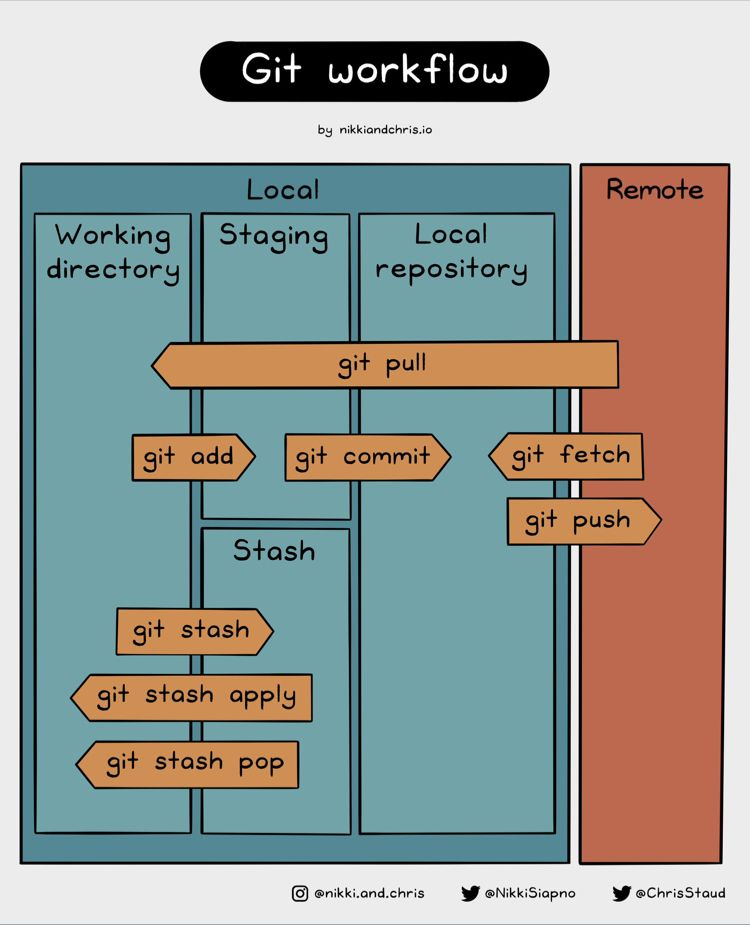
\includegraphics{images/git-flow.png}

\hypertarget{why-use-git}{%
\subsection{why use git?}\label{why-use-git}}

git, used properly, will make sure that you never, ever, ever end up in
a situation where you lose code. If you make changes to your code, you
can go back in the commit history and find the last working version. if
you accidentally delete everything, git will let you recover it. if your
computer gets blown up, your code is backed up. If you're working on a
collaborative project, git will help you resolve issues when you and
your collaborators modify code at the same time.

\hypertarget{basics}{%
\subsection{basics}\label{basics}}

git is supposed to be simple, but can often feel anything but. Here are
the 7 absolute basic commands you need to know:

\begin{itemize}
\tightlist
\item
  \texttt{git\ help} \ldots prints help

  \begin{itemize}
  \tightlist
  \item
    note the commands: \texttt{git\ help\ tutorial},
    \texttt{git\ help\ everyday}, \texttt{git\ help\ workflows}
  \end{itemize}
\item
  \texttt{git\ clone\ \{url\}\ \{folder\}} clones the git repo at
  \texttt{\{url\}} into \texttt{\{folder\}}

  \begin{itemize}
  \tightlist
  \item
    \texttt{\{url\}} is usually a github link like
    \texttt{https://github.com/someuser/repositoryname}
  \item
    if \texttt{\{fname\}} is not given, it will clone into a directory
    with the name \texttt{\{repositoryname\}}
  \end{itemize}
\item
  \texttt{git\ status} shows you what's going on in the current
  repository
\item
  \texttt{git\ add\ \{files\}} ``stages'' files (selects them for being
  commited)
\item
  \texttt{git\ commit} ``commits'' your changes -- they are now added to
  the official list of changes
\item
  \texttt{git\ pull} synchronizes your client by pulling files from the
  remote
\item
  \texttt{git\ push} sends whatever changes you have commited to the
  remote
\end{itemize}

\hypertarget{details}{%
\subsection{details}\label{details}}

A ``git repository'' is a directory in which certain files are
\emph{tracked} by git. when you run any \texttt{git} command, it looks
for a \texttt{.git} file in the current directory, and recursively in
every parent directory. that folder contains the whole history of all
changes you've commited to the repository.

Your local history can synchronize with a ``remote''
repository\footnote{if you want to start a local-only git repository,
  you can run \texttt{git\ init} in a repository. this will create a
  \texttt{.git} folder, and start tracking changes. If you then want
  these to then be synced with the cloud, you will need to use
  \texttt{git\ remote\ add\ origin\ \{url\}}. for this tutorial, we
  assume the creation of a repository on github first{]}} -- this is the
primary way of backing up your code, and collaborating with others.
GitHub, GitLab, BitBucket, and other websites provide (free) hosting of
git repositories. We will be using GitHub in this tutorial.

\begin{itemize}
\tightlist
\item
  When you make changes, git does not automatically do anything
\item
  To track changes, you must first add them using
  \texttt{git\ add\ \{files\}} (\texttt{git\ add\ .} will add everything
  in the current directory)

  \begin{itemize}
  \tightlist
  \item
    you can exclude files via a special \texttt{.gitignore} file, which
    you may look up the documentation for. this is useful if you have
    built binaries that you dont want to upload, have files with API or
    SSH keys you don't want to make public, or have a bunch of data that
    you don't want to upload.
  \end{itemize}
\item
  When you run \texttt{git\ status}, it will show you which changes have
  been added and which have not
\item
  when you run \texttt{git\ commit}, it will add all the changes along
  with your message to a ``tree''
\end{itemize}


\includegraphics{mermaid-images/20b80f24a3a6ddcdc2db54e00763d5117b2df660.png}

\hypertarget{branching}{%
\subsubsection{branching}\label{branching}}

When you're working on code with other people, want a persistent version
of your code that is always functional, or otherwise need multiple
versions of your code, branches are your friend. Git handles history as
a ``tree'', where the main trunk is called \texttt{main} (somtimes
\texttt{master} on older systems), and you can branch off at any commit.
After making changes, you can then re-merge the branch


\includegraphics{mermaid-images/74e31f8c420d1a7efbaf236e6b27b99455a87800.png}

key commands:

\begin{itemize}
\tightlist
\item
  \texttt{git\ branch} see the active branches
\item
  \texttt{git\ branch\ \{name\}} create a new branch
\item
  \texttt{git\ checkout\ \{name\}} switch to a branch
\end{itemize}

merging branches in the command line is possible, but I'll be covering
how to do it in the github client

\hypertarget{github}{%
\subsection{github}\label{github}}

Github is a platform for hosting git repositories. It is free, and has a
lot of features. You can find other peoples's code, ``fork'' it (make a
copy that belongs to you), make changes, and then merge your changes
into the original repository. It also acts as a sort of social network
for anything code-related, and having some open source projects up on
your github can be a great way to stand out to employers.

The main thing to know about what github adds is \textbf{Pull
Requests}:\\
A pull request ``pulls'' changes from one branch onto another branch --
this terminology can be confusing, but in the interface the ``source''
branch is on the right and the ``target'' branch is on the left.

Github also supports various CI/CD features, which let you automatically
run code upon certain actions, like creating a pull request to the main
branch. These are beyond the scope of this bootcamp, but I'm happy to
chat about them sometime.

\hypertarget{branches}{%
\subsection{branches}\label{branches}}

\hypertarget{assignment}{%
\section{Assignment}\label{assignment}}

(try to do this all in the command line)

\begin{enumerate}
\def\labelenumi{\arabic{enumi}.}
\tightlist
\item
  install bash and git, if you haven't already
\item
  go to \href{https://github.com}{github.com} and create an account if
  you don't have one

  \begin{enumerate}
  \def\labelenumii{\arabic{enumii}.}
  \setcounter{enumii}{2}
  \tightlist
  \item
    log in to github on your system. this will vary depending on your
    OS, and you may have to generate a token on the website
  \end{enumerate}
\item
  fork and clone your fork of the repository
  \url{https://github.com/mivanit/bash-git-bootcamp}
\item
  change to the ``user-dev'' branch
\item
  navigate to the ``userdata'' folder
\item
  create and enter folder with your mines username
\item
  make some changes here -- write a script, add a file, whatever you
  want
\item
  add, commit, and push your changes
\item
  merge your changes with the \texttt{user-dev} branch on my repository
\end{enumerate}

\hypertarget{takeaways}{%
\section{Takeaways}\label{takeaways}}

\begin{itemize}
\tightlist
\item
  bash is useful for talking to computers and manipulating filesystems
  at scale
\item
  git and github will prevent you from ever losing your code
\end{itemize}

\hypertarget{resources}{%
\section{Resources}\label{resources}}

\begin{itemize}
\tightlist
\item
  \href{https://git-scm.com/doc}{git docs}
\item
  \href{https://devdocs.io/bash/}{bash docs}
\item
  \href{https://oit.ua.edu/wp-content/uploads/2020/12/Linux_bash_cheat_sheet-1.pdf}{bash
  cheat sheet} (there are many online)
\item
  \href{https://pandoc.org/MANUAL.html}{pandoc}
\item
  how to use git in the command line is good to know, but there are many
  graphical interfaces for it. I reccomend
  \href{https://desktop.github.com}{GitHub Desktop}
\end{itemize}

\printbibliography

\end{document}
